\documentclass{sigchi}

\usepackage{balance}  % to better equalize the last page
\usepackage{graphics} % for EPS, load graphicx instead
\usepackage{times}    % comment if you want LaTeX's default font
\usepackage{url}      % llt: nicely formatted URLs

\toappear{}

\graphicspath{{graphics/}} 

% llt: Define a global style for URLs, rather that the default one
\makeatletter
\def\url@leostyle{%
  \@ifundefined{selectfont}{\def\UrlFont{\sf}}{\def\UrlFont{\small\bf\ttfamily}}}
\makeatother
\urlstyle{leo}

% To make various LaTeX processors do the right thing with page size.
\def\pprw{8.5in}
\def\pprh{11in}
\special{papersize=\pprw,\pprh}
\setlength{\paperwidth}{\pprw}
\setlength{\paperheight}{\pprh}
\setlength{\pdfpagewidth}{\pprw}
\setlength{\pdfpageheight}{\pprh}

% Make sure hyperref comes last of your loaded packages, 
% to give it a fighting chance of not being over-written, 
% since its job is to redefine many LaTeX commands.
\usepackage[pdftex]{hyperref}
\hypersetup{
  pdftitle={Fitness Adventure: an interactive floor game to maintain body fitness},
  pdfauthor={LaTeX},
  pdfkeywords={HCI, fitness, floor, adventure},
  bookmarksnumbered,
  pdfstartview={FitH},
  colorlinks,
  citecolor=black,
  filecolor=black,
  linkcolor=black,
  urlcolor=black,
  breaklinks=true,
}

% create a shortcut to typeset table headings
\newcommand\tabhead[1]{\small\textbf{#1}}

% End of preamble. Here it comes the document.
\begin{document}

  \title{Fitness Adventure: an interactive floor game to maintain body fitness}

  \author{
    \alignauthor Carl Ambroselli, Marc-Philipp Bismar, Marvin Bornstein, Julius Treike\\
    \affaddr{Hasso-Plattner-Institut}\\
    \affaddr{Potsdam, Germany}\\
    \email{\{carl.ambroselli, marc-philipp.bismar, marvin.bornstein, julius.treike\}@student.hpi.de}
  }

  \maketitle

  \begin{abstract}
    We introduce a jump 'n' run game for interactive floors to maintain body fitness. Players control themselves directly by stepping, jumping or laying on the floor. In a forrest, users jump over fallen trees or cross an ocean by holding themselves on ice floes. Repairing a bridge in shortage of time or similar complex tasks pack fitness exercises in an exciting adventure. This motivates users to do regular physical activity.
  \end{abstract}

  \section{Introduction}
    Most of today's tasks are done by machines. The majority of people spend almost the whole day in an office -- sitting.
    Fitness apps for smartphones are getting more and pupular and many people subscripe to local fitness centres. 
    At least the persons we asked about their sports activity in our contextual inquery. 

    \begin{figure}[ht]
      \centering
      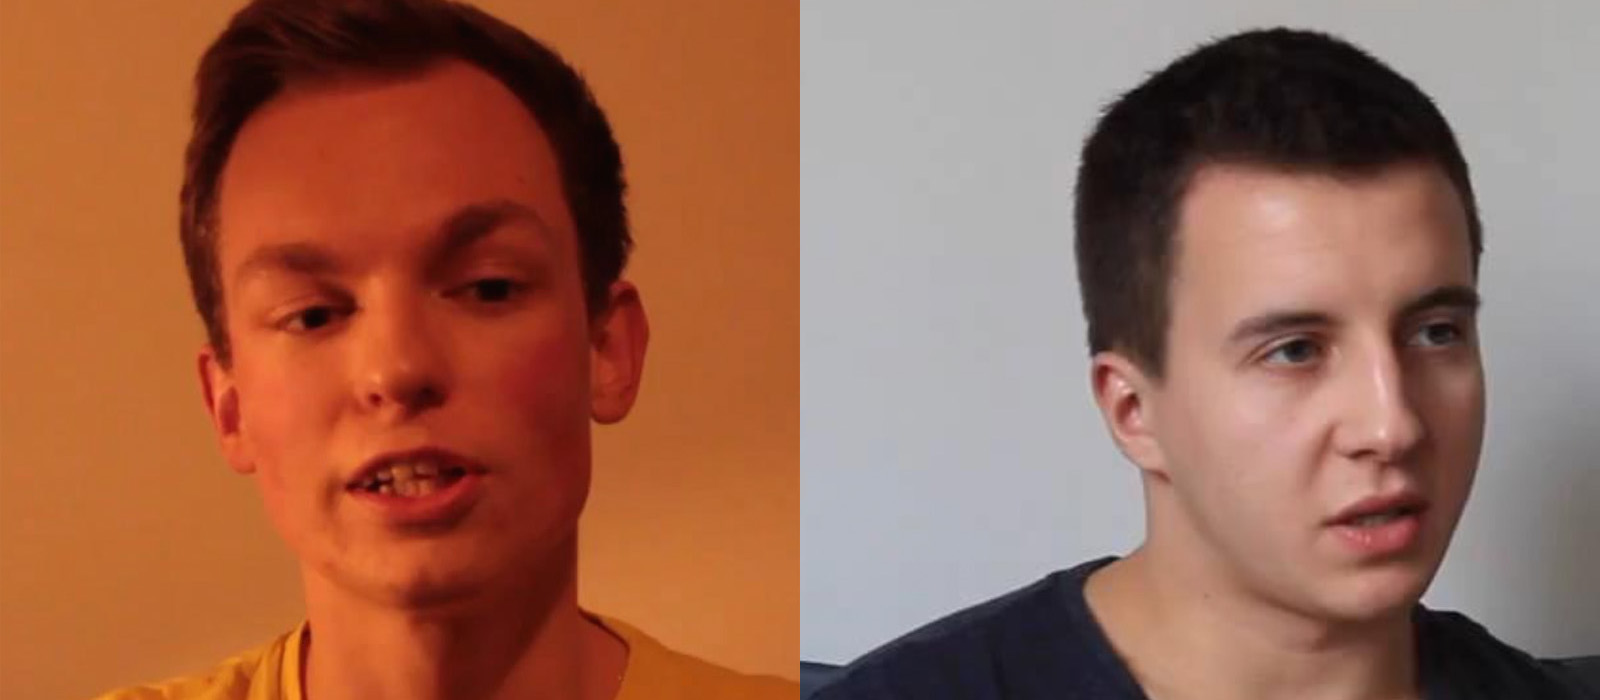
\includegraphics[width=\columnwidth]{users_casual}
      \caption{Interviewees with casual sports background. Justus Wirth (left) and Markus Petrykowski (right)}
      \label{fig:users_casual}
    \end{figure}

    \begin{figure}[ht]
      \centering
      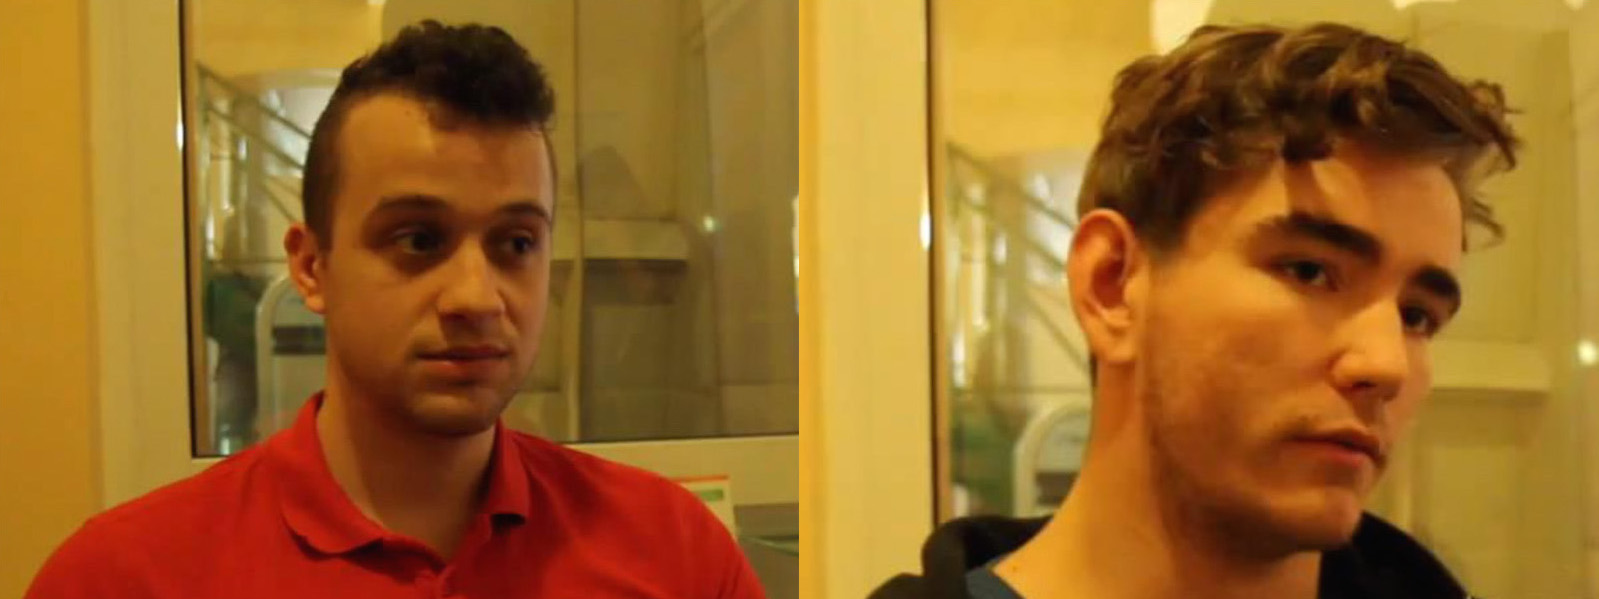
\includegraphics[width=\columnwidth]{users_pro}
      \caption{Interviewees with professional sports background. Ruben Zieger (left) and Carl Link (right)}
      \label{fig:users_pro}
    \end{figure}

    Markus (Figure \ref{fig:users_casual} on the right) studies computer science in Potsdam and has not much time for doing sport. In order to be balanced and healthy, he goes swimming or climbing once a week. He wants a flexible, non-complex and short exercise pack. A notable training progress would be a great motivation.

    Justus Wirth (Figure \ref{fig:users_casual} on the left) started doing freelethics in order to maintain health and get a better body. He wants to improve his performance in every training session and somehow get feedback on how well he performed his exercises.

    Carl and Ruben (Figure \ref{fig:users_pro}) from the \emph{Fit in Friedrichshain} fitness centre do bodybuilding on a professional level. Their motivations are also their bodies as well as their jobs. In general the motivation really depends on the individual person. Their clients, however, already bring the necessary motivation. Both, Carl and Ruben, were very interested in the idea of a touch floor exercising application, but mentioned problems regarding gym equipment. ``\emph{Every kind of activity is good.}'' says Carl, ``\emph{but there are no effective exercises for training the shoulders for example}''. 

    As a result, we focus on regular activity, instead of building up muscles and offer another approach to motivate activity: a video game. Users embody the protagonist themselves, explore the world and beat their own highscores by completing the level faster. This enables users to improve on every ``\emph{training}'' and also requires more energy and endurance. In addition, the game offers another environment for exercises than the traditional fitness studio and thus addresses other kinds of people.

  \begin{figure}[!t]
    \centering
    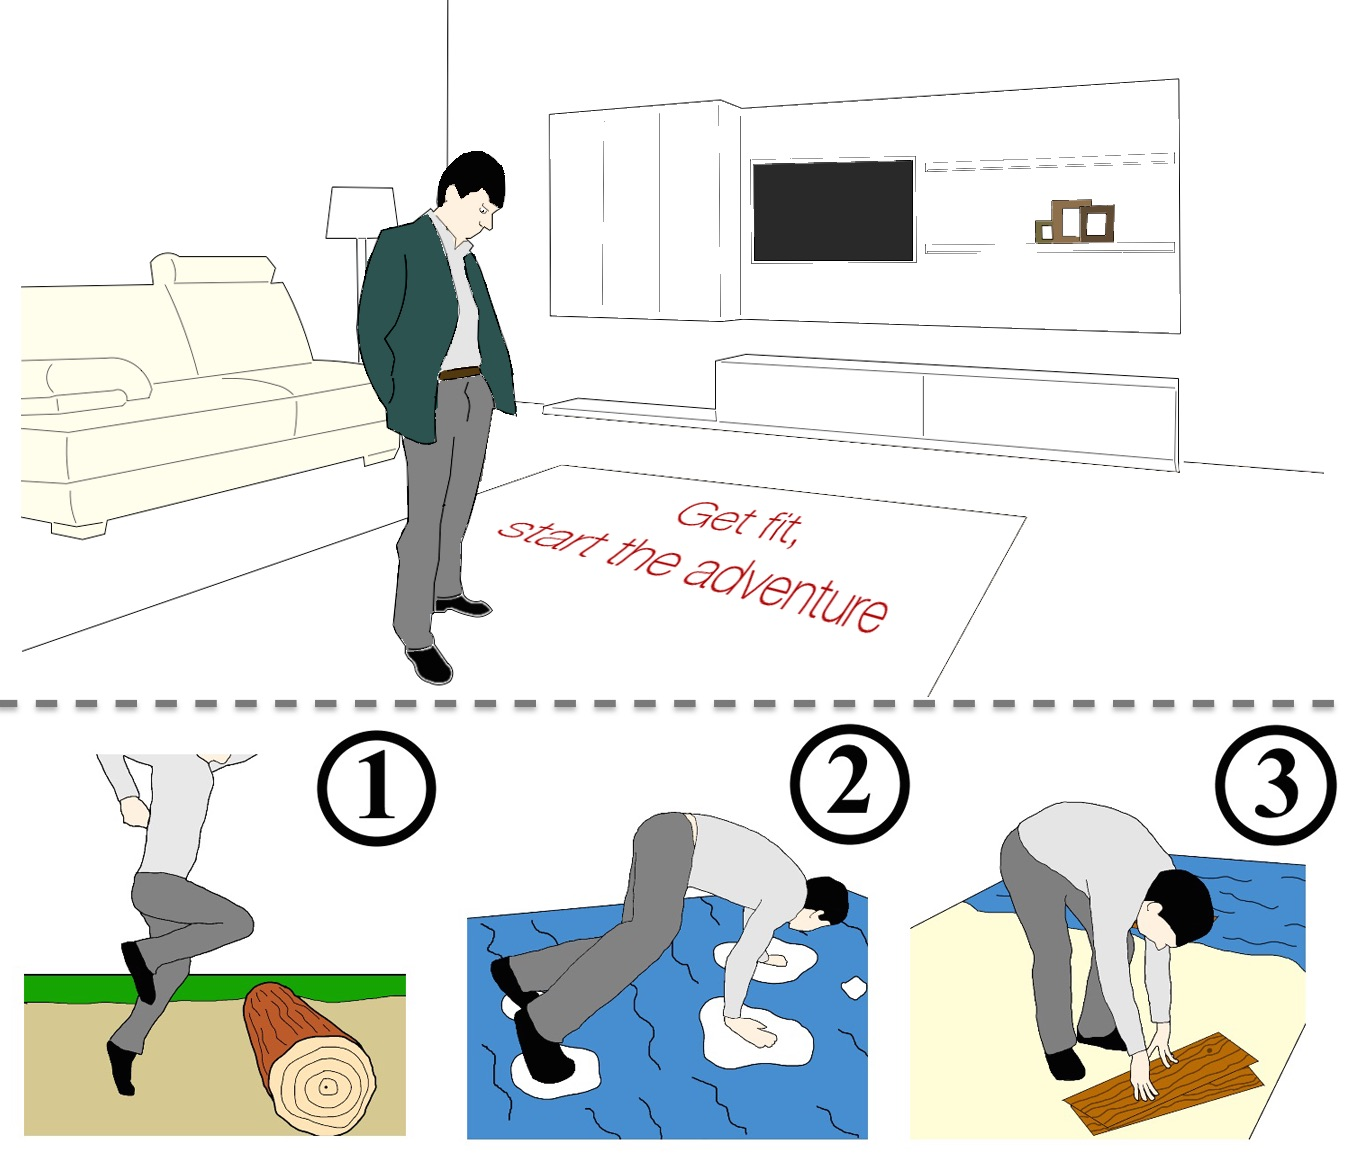
\includegraphics[width=\columnwidth]{roto_main}
    \caption{doing sport exercises on an interactive floor as part of the game}
    \label{fig:figure1}
  \end{figure}


\section{Walkthrough}

  In this scenario the student Andy trains his body by running in place, jumping a lot, staying in push-ups position and alternating running and touching the floor.

  \begin{figure}[!htb]
  \minipage{0.5\textwidth}
    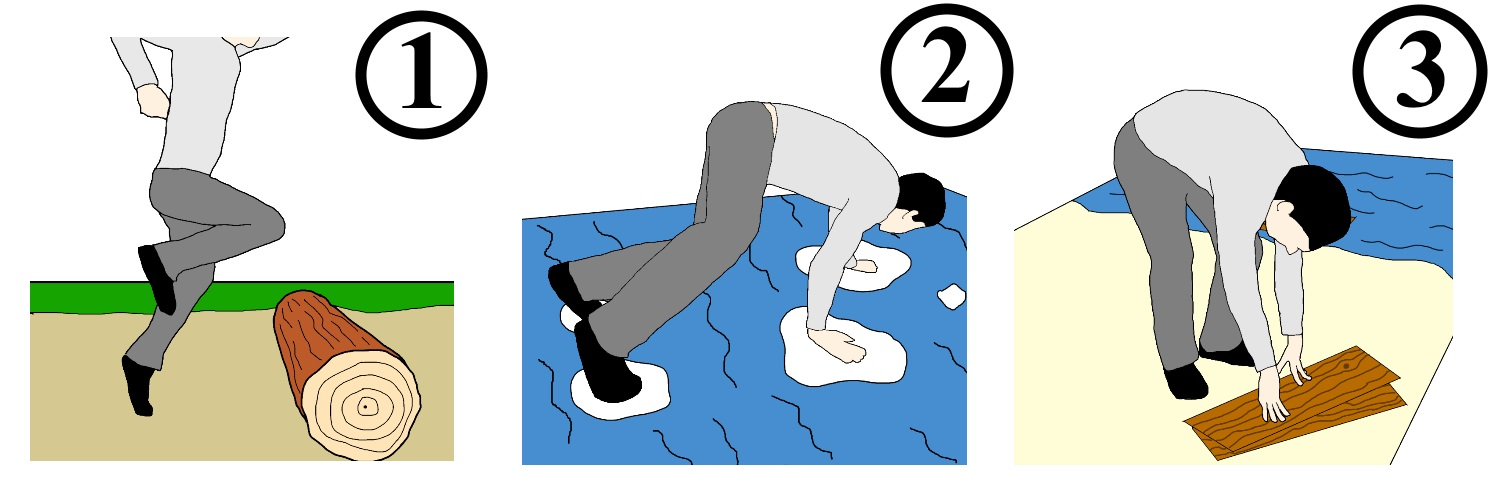
\includegraphics[width=\linewidth]{Image_11.jpg}
  \endminipage\hfill
    \caption{Task Overview. (1) Andy runs in place and jumps over trees. (2) Water appeared  with some ice floes on it and Andy has to stay on these, but they melt. (3) Andy has to build a bridge to cross the water.}\label{fig:awesome_image3}
  \end{figure}

  The conrete beginning of the game (Figure 3 (1)) includes more thoughts. We focus on it in detail.

  \begin{figure}[!htb]
  \minipage{0.5\textwidth}
    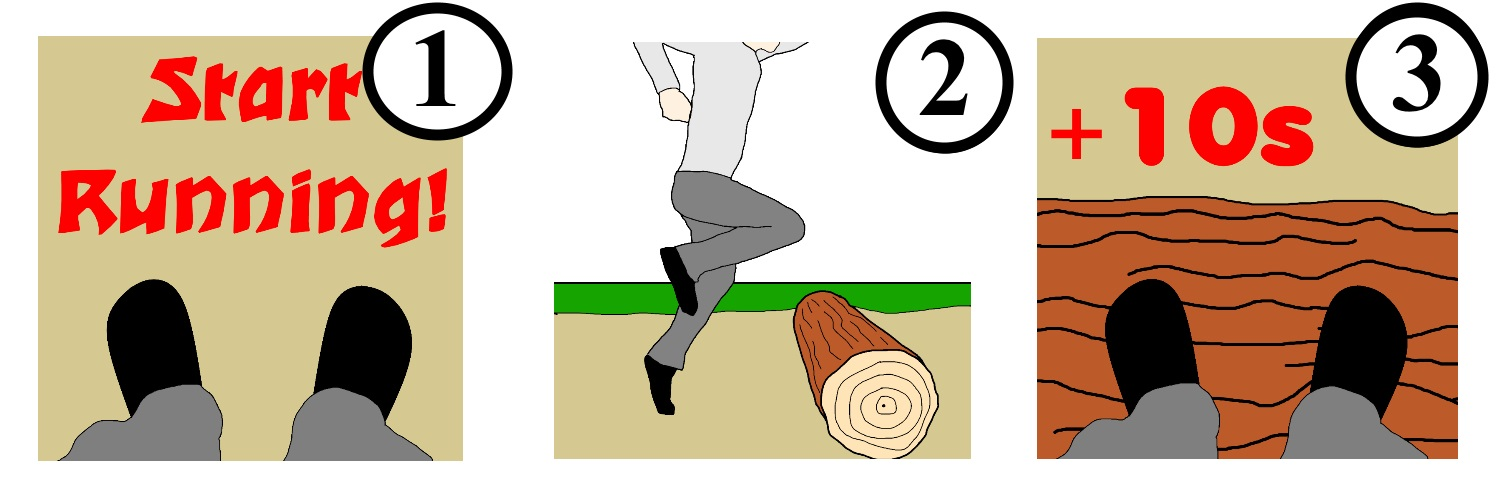
\includegraphics[width=\linewidth]{Image_12.jpg}
  \endminipage\hfill
    \caption{(1) Andy is entering the floor and immediatly instructed to start running. The floor will begin to move under his feet. (2) When trees appear on the way, Andy has to jump over them. (3) When Andy unintentionally lands on a tree, he is punished with extra time (time is counting forwarsds and stopped, when one run is finished).}\label{fig:awesome_image3}
  \end{figure}

  \begin{figure}[!htb]
  \minipage{0.5\textwidth}
    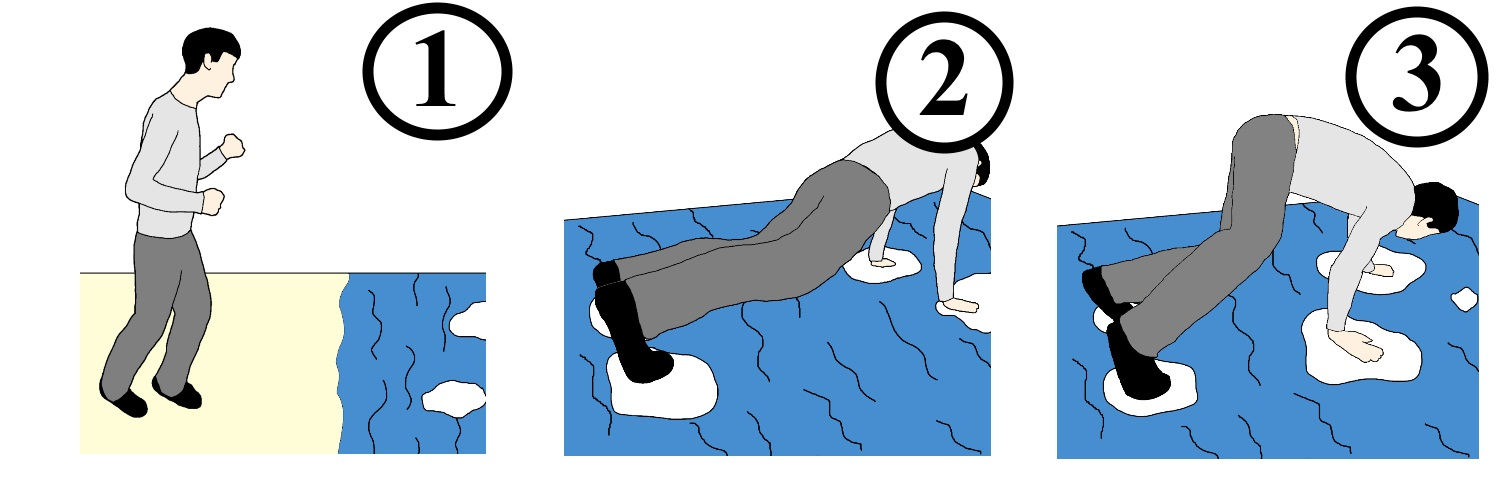
\includegraphics[width=\linewidth]{Image_13.jpg}
  \endminipage\hfill
    \caption{(1) Andy runs over a beach and approaches water with ice floes on it. He is instructed to jump on them. (2) After jumping on the icefloes, he put his hand onto the other ice floes. (3) When an ice floe melts, others appear, Andy has to put the hand on.}\label{fig:awesome_image3}
  \end{figure}

  After a the ice floe game, the run proceeds as already shown in figure 3.

  \begin{figure}[!htb]
  \minipage{0.5\textwidth}
    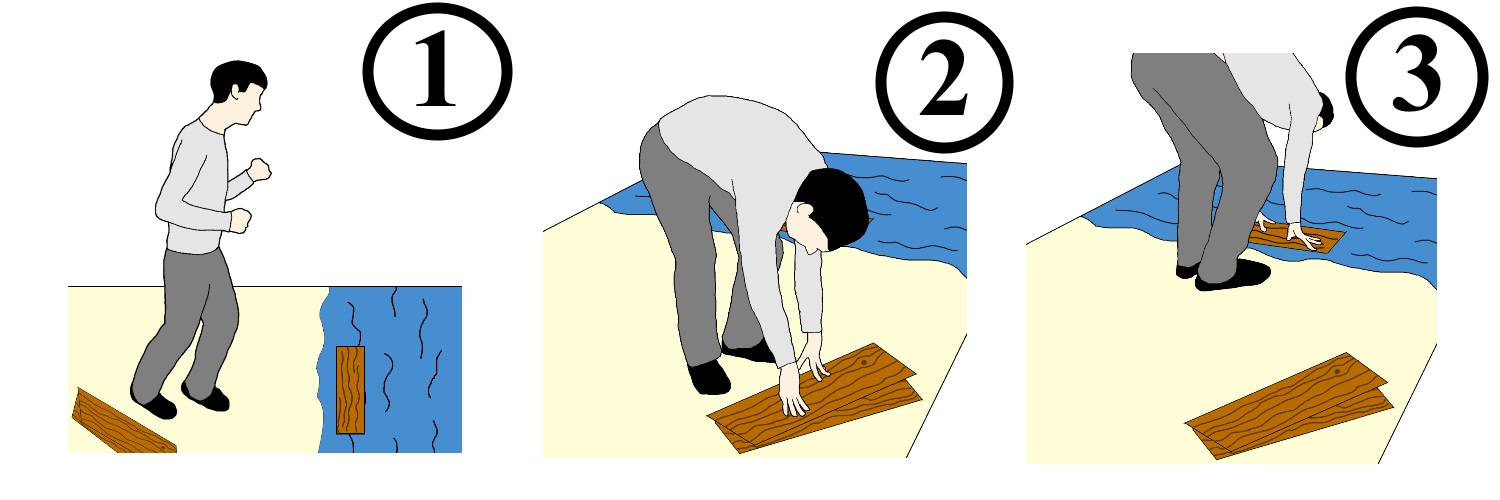
\includegraphics[width=\linewidth]{Image_14.jpg}
  \endminipage\hfill
    \caption{(1) Andy runs over a beach with wood planks and is instructed to build a bridge to cross the water. (2) Andy touches the floor with his hands on the woodplanks to collect one. (3) He touches the water to build a part of a bridge. (4) Andy did alternating (2) and (3), finished the bridge and proceeds his run.}\label{fig:awesome_image3}
  \end{figure}

\section{Design}

  \subsection{Instantly start game}

    We had several iterations when to start a workout. Ideas like special locations like fitness mat turned out to be bad since the user did not understand them  when testing with a paper prototype. In the final version we chose to start the game as soon as someone starts running on the floor to provide the simplest   solution as possible.

    During heuristic evaluation we identified that there must be a short message telling the user that he should start running, from that point on he understood  how to start a workout and make progress.

  \subsection{Dictate Exercises}

    In the early designs, we decided to let users choose the exercise they want to do and guide them in their performance. Possible tasks were to train you legs  for n seconds or build up strength performing n short, but hard exercises.

    Within tast analysis, we noticed that this violates the need for a short workout, because much time is spent in the menu on selecting workouts. In our paper  prototype study two out of our 3 participants did not even know what the exercises are about or what kind of training they are. Users rather wanted to be     guided and told what would be best to do.

    In the further process we reduced the options down to only 'warmup' or 'workout'. In the final design, we have a complete world with several workouts packed  in mini games.


\section{Conclusion}

  When designing applications for interactive floors, user studies and exploration with prototypes becomes extremely imporant since there are no general patterns and the problem domain is yet unexplored. During the process our evaluation of the user's needs changed radically. When asking users what they wanted they looked at existing solutions and tried to map them to the floor. If we followed those, we would have ended up with a fitness mat and a video player. But this is already the solution for people, who want to do fitness without any sport equipment. We collected important aspects from users like the need for motivation and limited free time and mapped them to possible exersices on the floor. Finally we came to the conclusion, that games are the most interactive solution that motivate users with fun when they work out. The ability to challenge your high score pushes your goals and shows you your progress. 
    Since developing an interactive protoype for a floor requires a major amount of work, paper prototyping turned out to be a powerful tool to find design flaws in your prototypes as users were able to imagine the system.
    In addition, even when users want to use an application to do fitness activity, they look for the simplest solution to solve a game. Therefore you need to design fitness games that force users to do certain activity with the desired path instead of giving them the freedom how they want to solve a certain task.

\end{document}